

\documentclass{report}

\usepackage[tc]{titlepic}
\usepackage[utf8x]{inputenc}
\usepackage[french]{babel}
\usepackage{graphicx}
\usepackage{geometry}
\usepackage{ifthen}
\usepackage{enumerate}

\graphicspath{{fig/}}

\newcommand\Titre{Devoir 2}
\newcommand\Auteur{Maxence Caron, Jules Caron, Hugues Soares}
\newcommand\Destinataire{Ronald Beaubrun}
\newcommand\NomEquipe{GLO-2000}
\newcommand\DateRemise{\today}


\geometry{letterpaper,%
          centering,%
          hmargin={2.5cm,2.5cm},%
          vmargin={2.5cm,2.5cm},%
          heightrounded,%
	  includehead}


\newenvironment{thebibliographyUL}[1]%
               {\clearpage%
                \begin{thebibliography}{#1}%
                \addcontentsline{toc}{chapter}{\bibname}%
                \raggedright%
               }%
               {\end{thebibliography}}

\renewcommand\maketitle{
	\thispagestyle{empty}%
	\pagenumbering{roman}%
	\begin{titlepage}%
		\setcounter{page}{999}%
		\begin{flushleft}
			
\includegraphics[width=12em]{ul_logo}
		\end{flushleft}\par
		\vspace*{\stretch{1}}
			\centering
			\parbox{\textwidth}{\centering\Large\bfseries \Titre}         \\[5ex]
			\vspace*{\stretch{2}}
			pr\'{e}sent\'{e} \`{a}                    \\[1ex]
			\textbf{\Destinataire}                 \\
			\vspace*{\stretch{1}}
		par                                       \\[1ex]
			{\large \'{E}quipe \NomEquipe}                \\[1ex]
			\Auteur\\[1ex]
			\vspace*{\stretch{1}}
			{\large Universit\'{e} Laval}             \\
			\DateRemise\\
	\end{titlepage}
}

% No section numbering
\makeatletter
\def\@seccntformat#1{%
  \expandafter\ifx\csname c@#1\endcsname\c@section\else
  \csname the#1\endcsname\quad
  \fi}
\makeatother

% Definition du niveau hierarchique maximum couvert par la table des matieres
\setcounter{tocdepth}{3}            % default = 2

% Definition du niveau hierarchique maximum ayant une numerotation
\setcounter{secnumdepth}{3}         % default = 2

\begin{document}

\maketitle
%\tableofcontents
%		\ifthenelse{\boolean{false}}%
%			{\clearpage%
%			\listoffigures%
%			\addcontentsline{toc}{chapter}{\listfigurename}}{}
%		\ifthenelse{\boolean{false}}%
%			{\clearpage%
%			\listoftables%
%			\addcontentsline{toc}{chapter}{\listtablename}}{}

\cleardoublepage%
\setcounter{page}{1}%
\pagenumbering{arabic}%

\chapter{Réseaux - devoir 2}

\section{Question 1 à 3}
\begin{figure}[h]
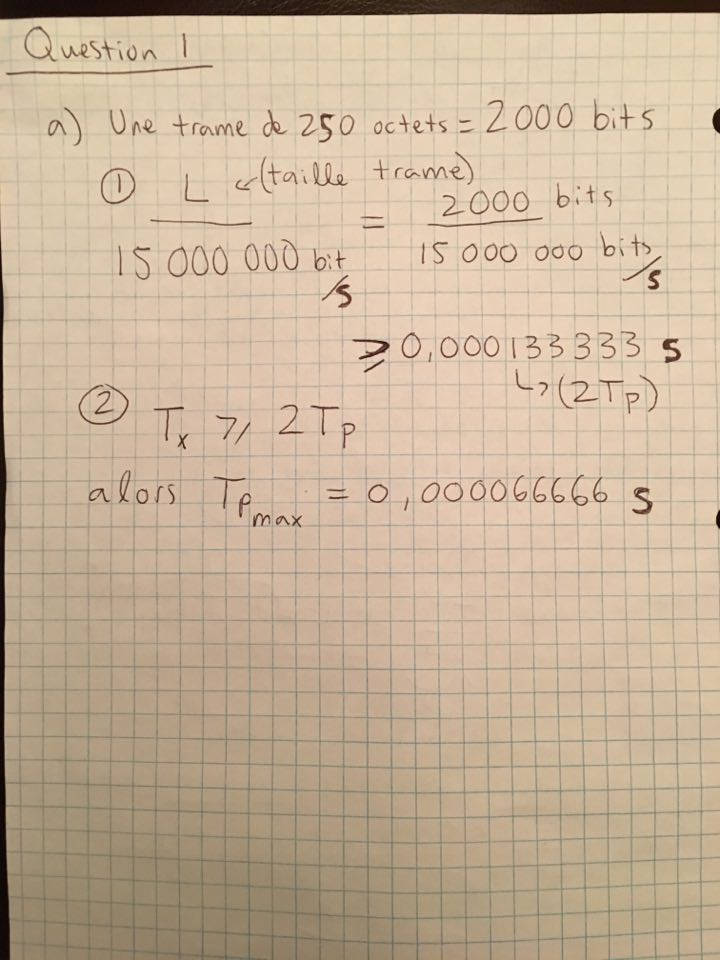
\includegraphics[scale=0.7]{1-1.jpg}
\end{figure}
\begin{figure}[h]
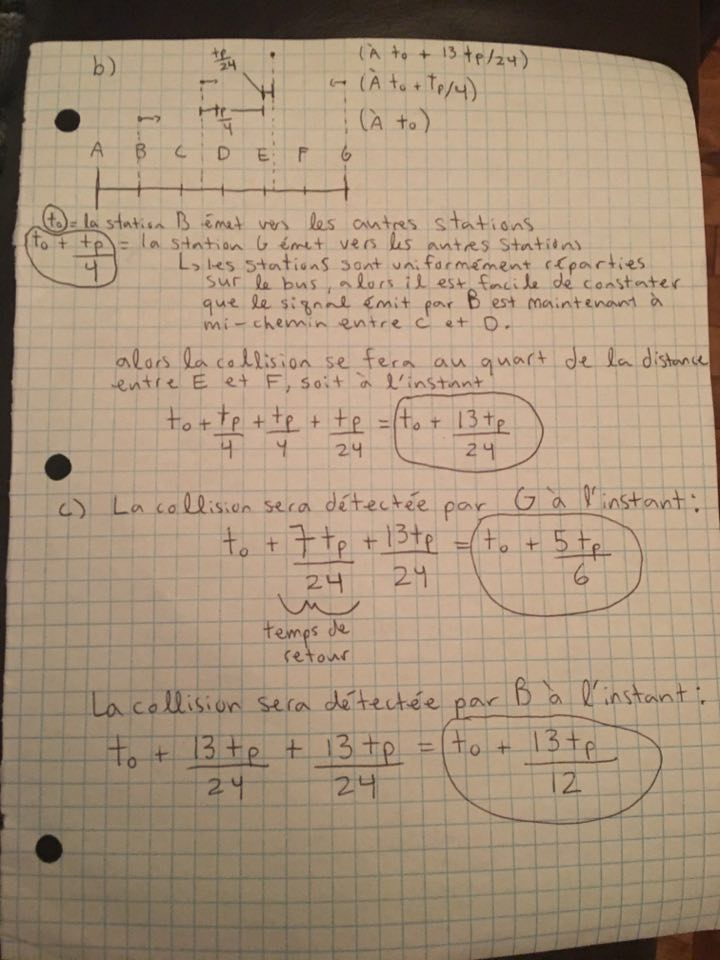
\includegraphics[scale=0.7]{1-2.jpg}
\end{figure}
\begin{figure}[h]
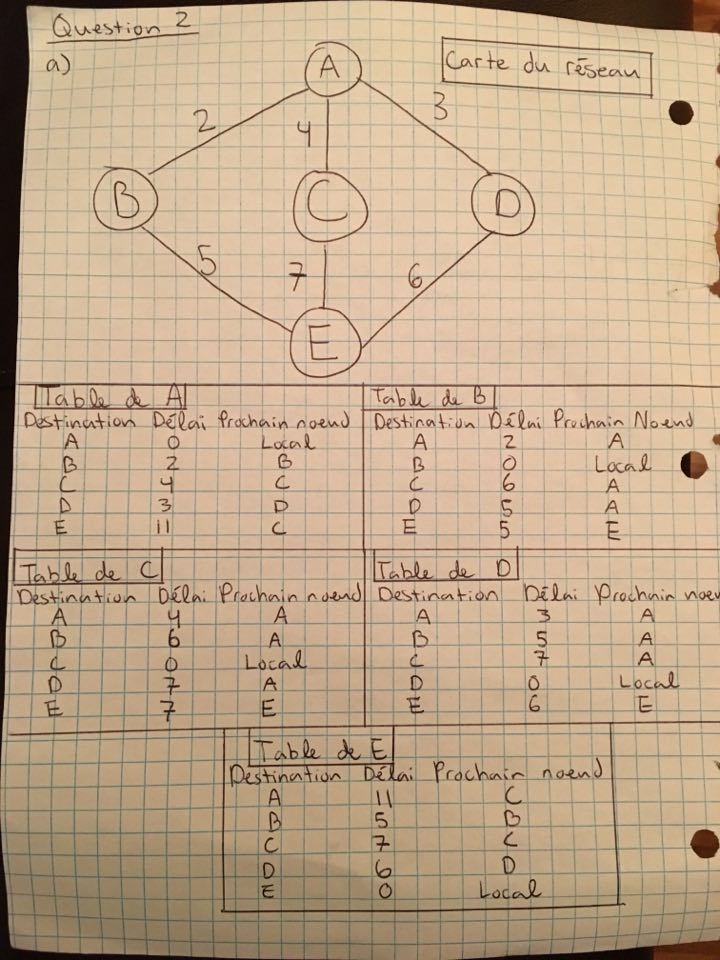
\includegraphics[scale=0.7]{2-1.jpg}
\end{figure}
\begin{figure}[h]
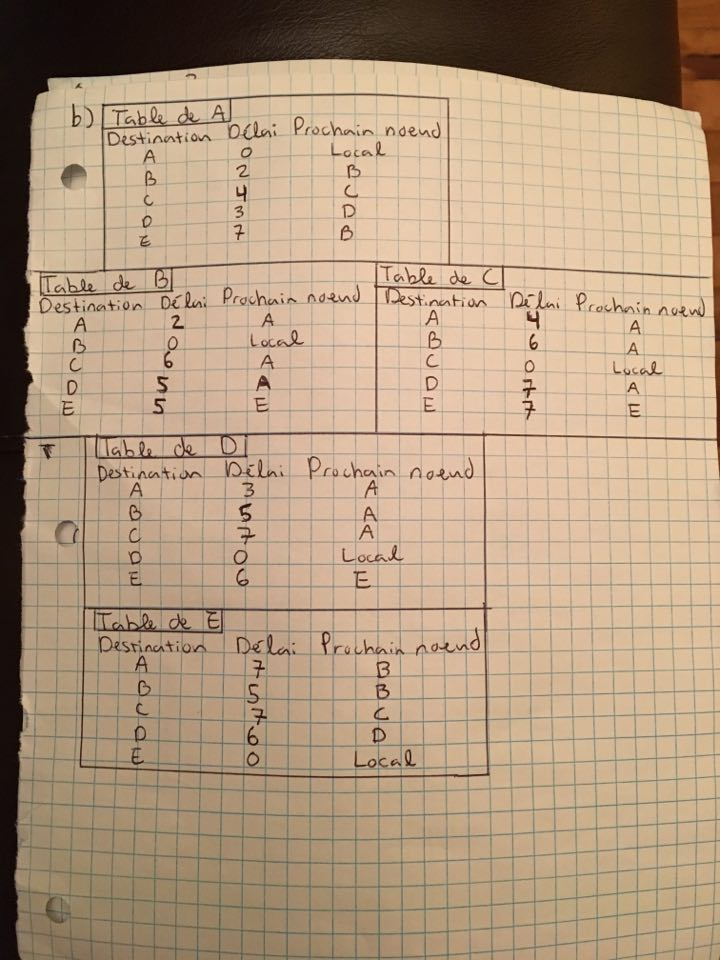
\includegraphics[scale=0.7]{2-2.jpg}
\end{figure}
\begin{figure}[h]
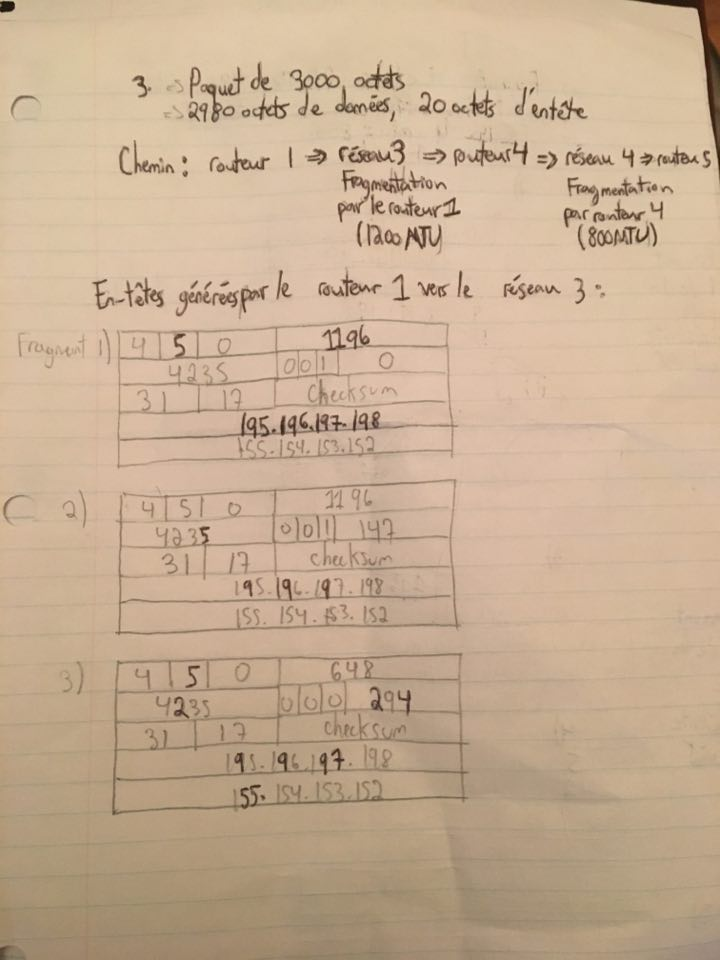
\includegraphics[scale=0.7]{3-1.jpg}
\end{figure}\begin{figure}[h]
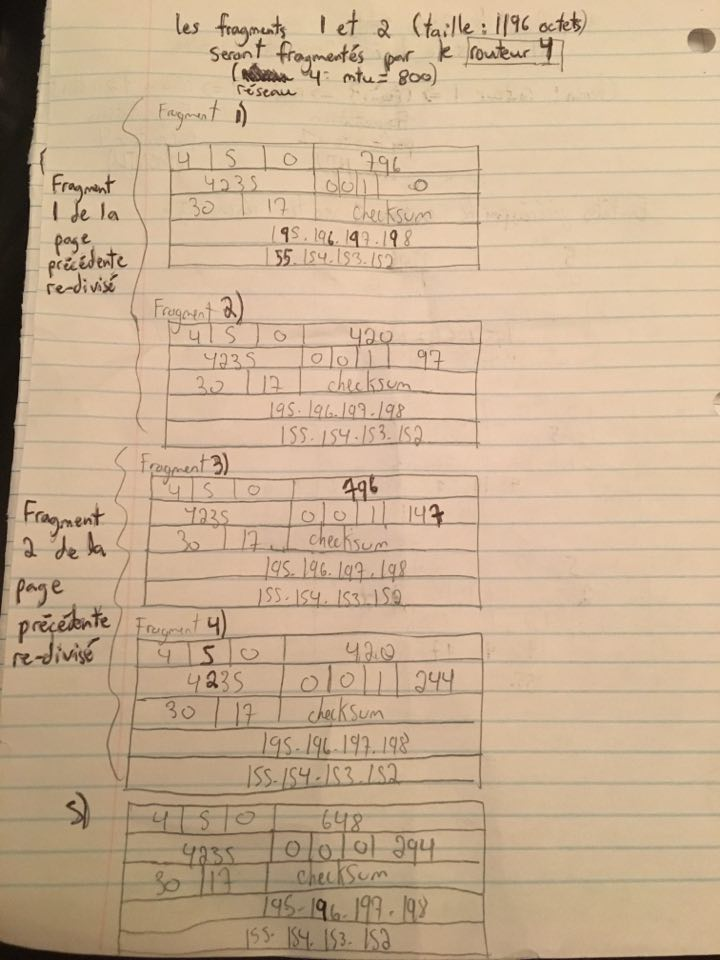
\includegraphics[scale=0.7]{3-2.jpg}
\end{figure}\begin{figure}[h]
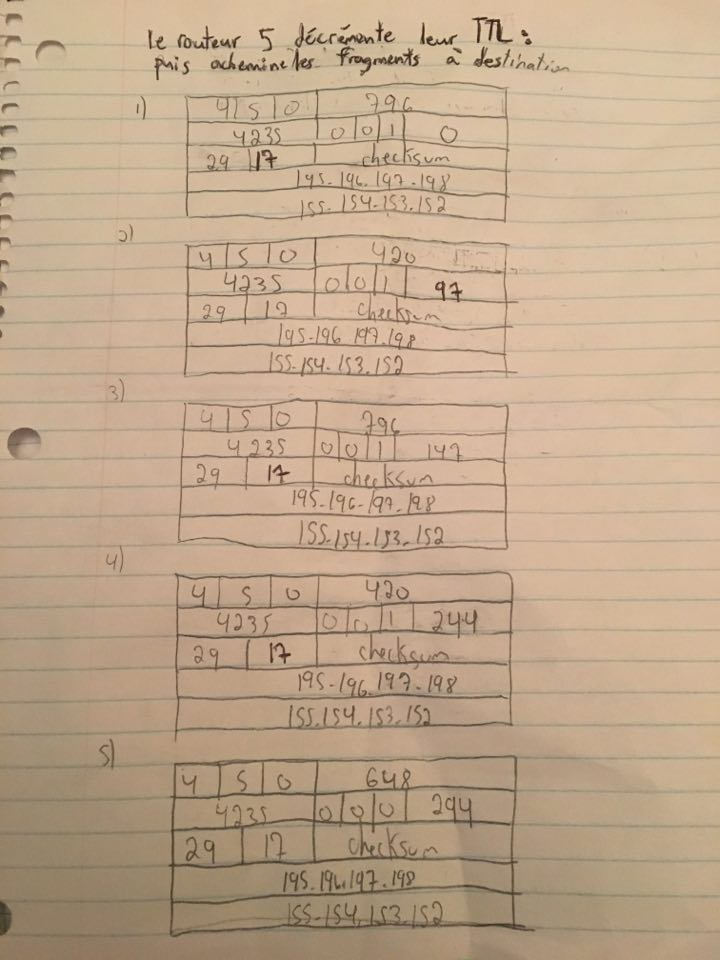
\includegraphics[scale=0.7]{3-3.jpg}
\end{figure}
\clearpage
\section{Question 4}
\begin{enumerate}[(a)]
	\item C'est une réseau de classe 'b' avec masque de sous réseau 
		par defaut : 255.255.0.0
	\item 255.255.254.0
	\item 138.123.0.0, 138.123.2.0, 138.123.4.0
	\item 138.123.250.0, 138.123.252.0, 138.123.254.0
	\item 138.123.10.0, 138.123.10.1, 138.123.10.2
	\item 138.123.10.253, 138.123.10.254, 138.123.10.255
\end{enumerate}



\end{document}

